% !Tex root=tb_icml_2018.tex

\section{Convergence of Deep Generative Model for Alternative Parameter Settings}
\label{sec:app:exp-algs}

Figure~\ref{fig-app:mnistexpt/convergence} shows the convergence of the introduced algorithms under different
settings to those shown in Figure~\ref{fig:mnistexpt/convergence}. Namely we consider $M=4, K=16$ for~\gls{PIWAE} and~\gls{MIWAE} 
and $\beta = 0.05$ for~\gls{CIWAE}.  These settings all represent tighter bounds than those of the main paper.
Similar behavior is seen in terms of the~\gls{IWAE}-64 metric for all algorithms.  \gls{PIWAE} produced
similar mean behavior for all metrics, though the variance was noticeably increased for $\log \hat{p}(x)$.
For~\gls{CIWAE} and~\gls{MIWAE}, we see that the parameter settings represent an explicit trade-off between
the generative network and the inference network:  $\log \hat{p}(x)$ was noticeably increased for both, matching
that of~\gls{IWAE}, while $-\textsc{KL}(Q_{\phi}(z \given x) || P_{\theta}(z \given x))$ was reduced.
Critically, we see here that, as observed for~\gls{PIWAE} in the main paper,~\gls{MIWAE} and~\gls{CIWAE} are able to
match the generative model performance of~\gls{IWAE} whilst improving the KL metric, indicating that they have learned
better inference networks.

\begin{figure*}[h]
	\centering
   	\begin{subfigure}[b]{0.33\textwidth}
        \centering
        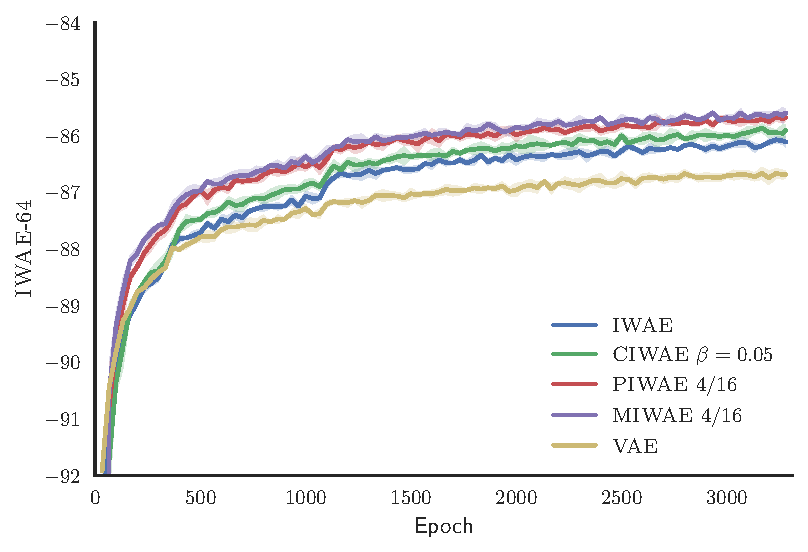
\includegraphics[width=\textwidth]{figures/tighter_bounds/optim_convergence_IWAE_64}
        \caption{\textsc{IWAE}$_{64}$ \label{fig-app:mnistexpt/convergence/iwae64}}
    \end{subfigure}
	\begin{subfigure}[b]{0.33\textwidth}
		\centering
		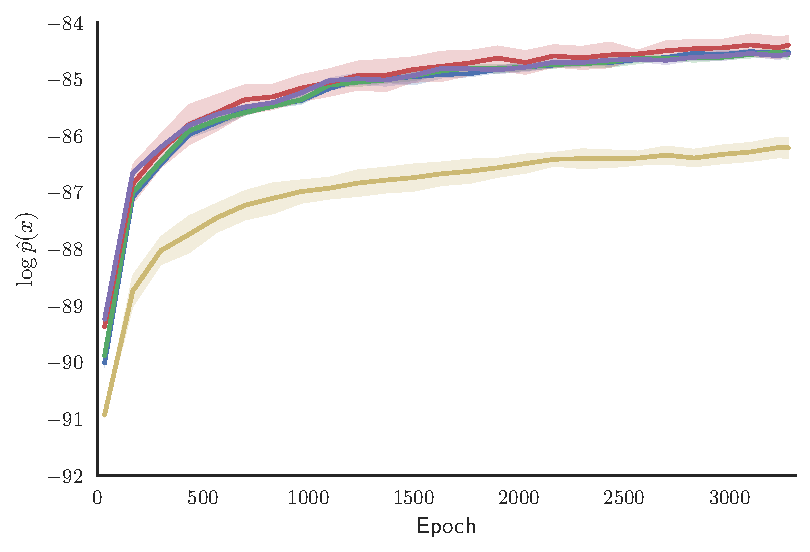
\includegraphics[width=\textwidth]{figures/tighter_bounds/optim_convergence_log_p(x)}
		\caption{$\log \hat{p}(x)$ \label{fig-app:mnistexpt/convergence/logpx}}
	\end{subfigure}
	\begin{subfigure}[b]{0.33\textwidth}
		\centering
		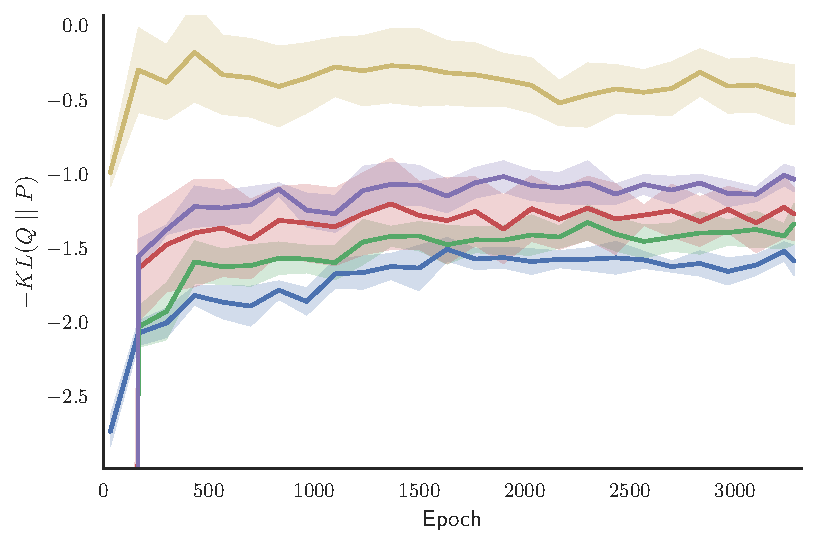
\includegraphics[width=\textwidth]{figures/tighter_bounds/optim_convergence_KL}
		\caption{$-\mathrm{KL}(Q_{\phi}(z \given x) || P_{\theta}(z \given x))$ \label{fig-app:mnistexpt/convergence/kl}}
	\end{subfigure}
	\caption{Convergence of different evaluation metrics for each method.  Plotting conventions as per
		 Figure~\ref{fig:mnistexpt/convergence}.
		\vspace{-12pt}  \label{fig-app:mnistexpt/convergence}}
\end{figure*}